\chapter{Containers}

Containers hold Items created by the User.
A Container created as Private cannot be changed to Shareable.
Similarly a Shareable Container cannot be changed to a Private Container.

\section{Create a Container}

From the Menu bar on top, select "Containers" tab and then select "Create new Container" from drop down menu.

\begin{figure}[H]
\centering
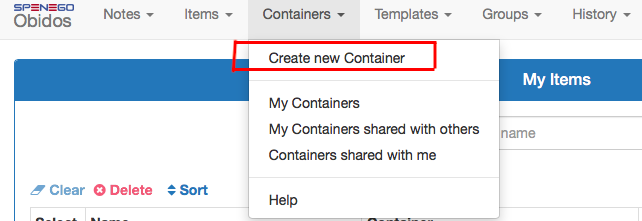
\includegraphics[width=90mm]{user/Create-Container.png}
\caption{"Create new Container" Menu}
\label{fig: Figure}
\end{figure}

In the 'Create Container' page, give a name for the Container. Specify the type of the Container, whether Shareable or Private. 

\begin{figure}[H]
\centering
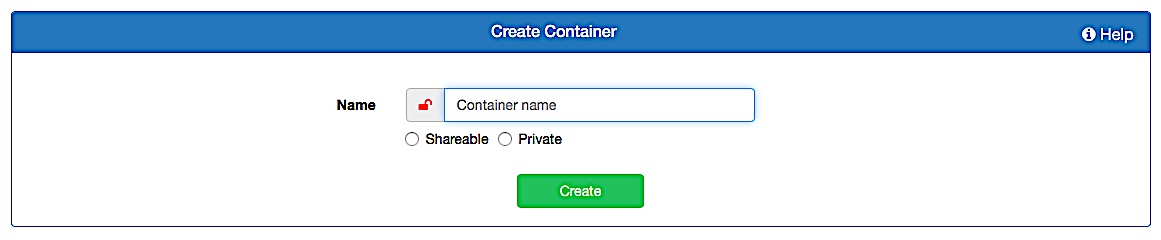
\includegraphics[width=150mm]{user/Create-Container-Frame.png}
\caption{Creating a Container}
\label{fig: Figure}
\end{figure}

\section{List Containers}

Select "My Containers" from the top "Containers" tab.
The list of Containers will be displayed in the format as shown in the following figure.

\begin{figure}[H]
\centering
\fbox{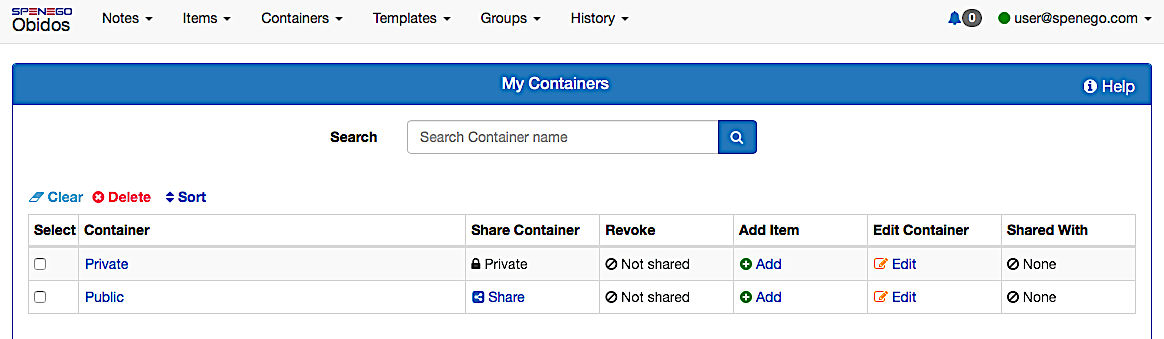
\includegraphics[width=180mm]{user/List-Containers.png}}
\caption{List of Containers}
\label{fig: Figure}
\end{figure}

\section{Delete a Container}

Select "My Containers" from the Container tab. A Container can be deleted only from this list.
Select the Container(s) to delete by clicking on the button to the left of the name(s) of the Container(s).
Then using the {\color{red}\faTimesCircle \ Delete} button on the top, the selected Container(s) can be deleted.
When a Container is deleted, all Items in the Container will be deleted. All Items shared from this Container will be revoked.

\begin{figure}[H]
\centering
\fbox{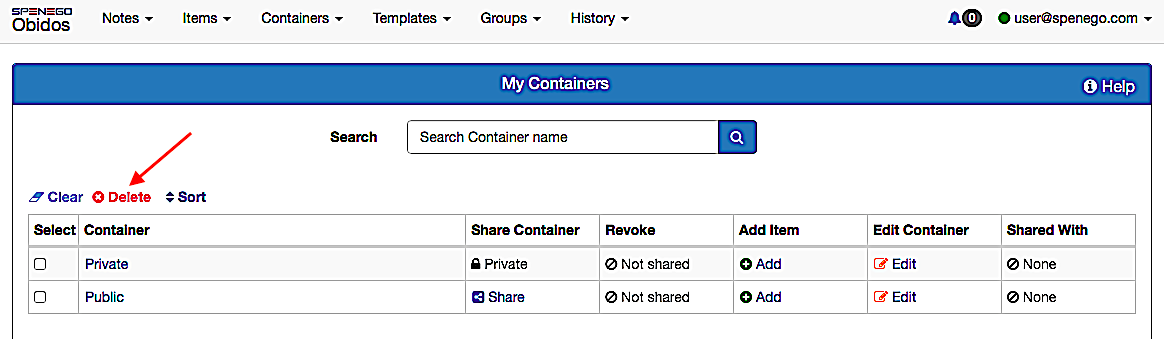
\includegraphics[width=180mm]{user/Delete-Container.png}}
\caption{Delete a Container}
\label{fig: Figure}
\end{figure}

\section{Share Container}
A Container can be shared only if it is of type Shareable.
Sharing a Container is done from "My Containers" list.

\begin{figure}[H]
\centering
\fbox{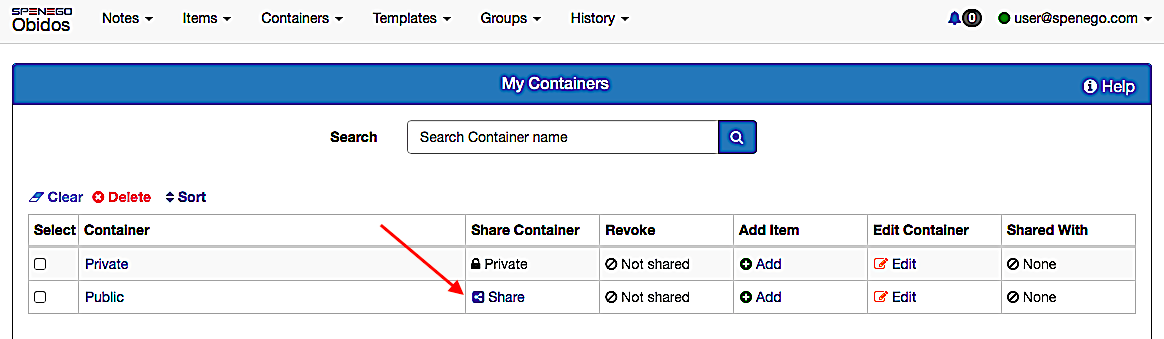
\includegraphics[width=180mm]{user/Share-Container.png}}
\caption{Sharing a Container}
\label{fig: Figure}
\end{figure}

Using the {\color{myblue}\faShareAltSquare \ Share} button on the line corresponding to the Container to be shared,
the sharing process can be initiated.

\section{Changing Name of a Container}
The name of a Container can be changed by editing it.
From "My Containers" list, use {\color{orange}\faEdit} {\color{myblue}Edit} link to initiate the edit process.

\begin{figure}[H]
\centering
\fbox{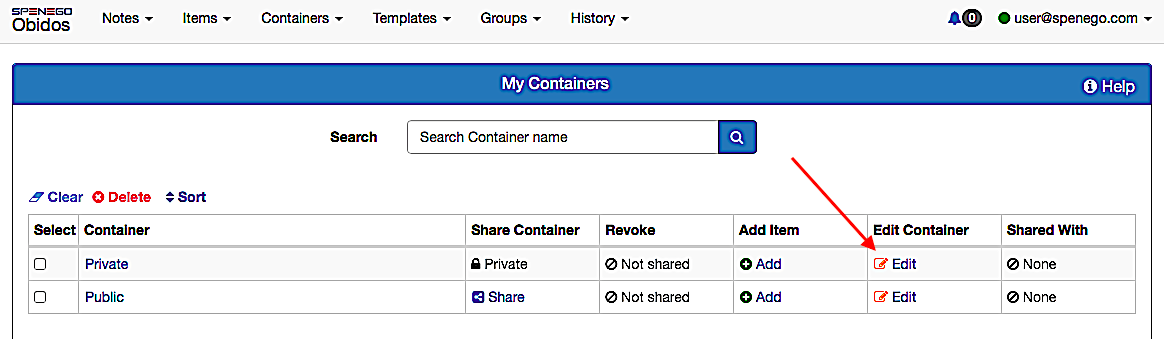
\includegraphics[width=180mm]{user/Edit-Container.png}}
\caption{Edit a Container}
\label{fig: Figure}
\end{figure}

On clicking {\color{orange}\faEdit} {\color{myblue}Edit} link, the screen to edit the Container will appear. 
There you will be able to change the name of the Container.
